\section{Τίτλος}

\begin{figure}[h!]
    \centering
    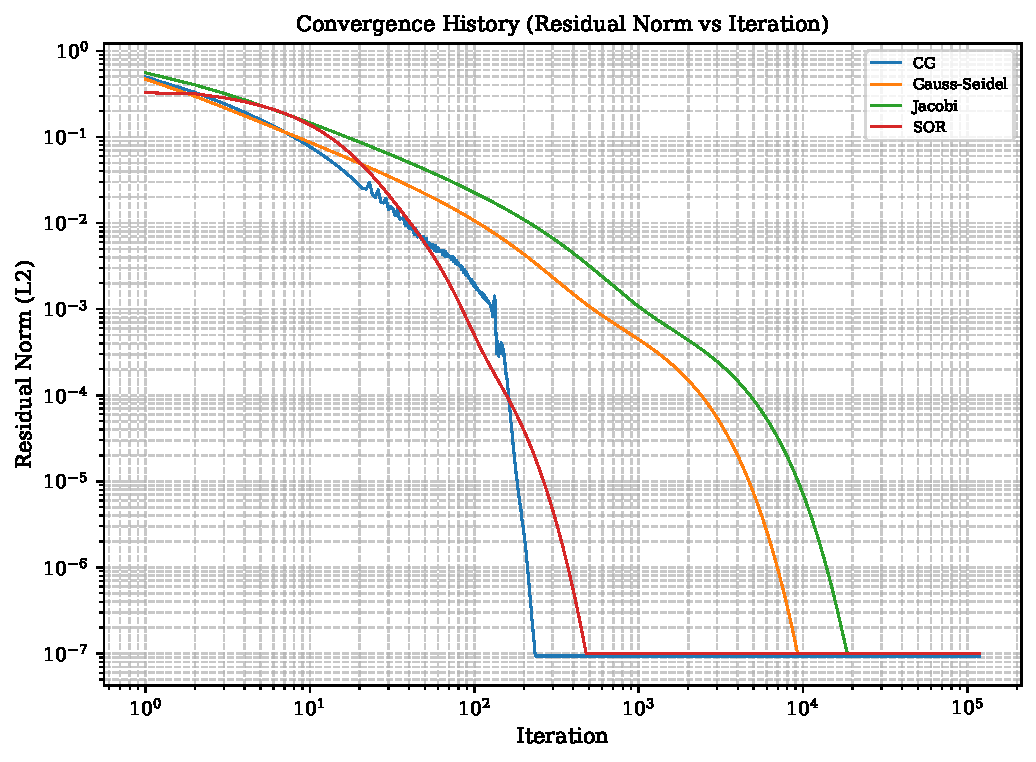
\includegraphics[width=0.60\linewidth]{doc/figures/convergence_plot.pdf}
    \caption{Σύντομη περιγραφή}
    \label{fig:placeholder}
\end{figure}

\begin{image}
    \centering
    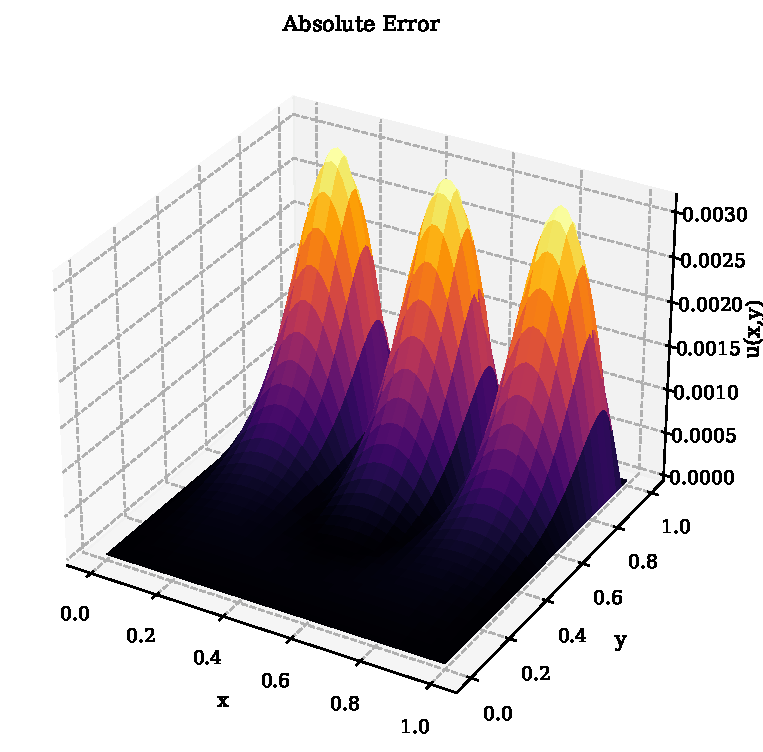
\includegraphics[width=0.50\textwidth]{doc/images/abs_error_surface.pdf}
    \caption{Σύντομη περιγραφή}
    \label{img:example}
\end{image}


\begin{table}[h!]
\centering
\begin{tabular}{|c|c|c|c|c|}
\hline
\en{N} & \en{CG} & \en{Gauss-Seidel} & \en{Jacobi} & \en{SOR} \\
\hline
0   & 8   & 14  & 64    & 35   \\
1   & 18  & 39  & 324   & 62   \\
2   & 28  & 64  & 784   & 87   \\
3   & 38  & 90  & 1444  & 112  \\
4   & 48  & 114 & 2304  & 136  \\
5   & 58  & 139 & 3364  & 161  \\
6   & 68  & 163 & 4624  & 225  \\
7   & 78  & 187 & 6084  & 304  \\
8   & 88  & 211 & 7614  & 388  \\
9   & 98  & 235 & 9260  & 479  \\
10  & 108 & 258 & 11048 & 577  \\
11  & 118 & 282 & 12977 & 682  \\
12  & 128 & 305 & 15043 & 794  \\
13  & 138 & 328 & 17244 & 913  \\
14  & 148 & 351 & 19577 & 1039 \\
15  & 158 & 374 & 22041 & 1172 \\
16  & 168 & 398 & 24633 & 1311 \\
17  & 178 & 421 & 27352 & 1457 \\
18  & 188 & 444 & 30196 & 1609 \\
19  & 198 & 467 & 33163 & 1768 \\
\hline
\end{tabular}
\caption{Σύντομη περιγραφή}
\label{tab:iteration_counts}
\end{table}